\chapter{Details about the Air-Water heat
  pump Prototype}
\label[secinapp]{chap:awp-components}
\resetallacronyms

\section{Components}
\label[secinapp]{sec:awp-components}

\subsection{Evaporator}
\label{awp-ev-details}

The evaporator\index{evaporator} of the \AWP{} was the evaporator set
in the housing provided by the industrial partner. That housing was
provided with the heat exchangers and an operational air channel and
fan. Those components were kept and used to design the \AWP{}.

\subsection{Pipes and fittings}
\label[secinapp]{sec:awp-pipes}

\begin{itemize}
\item Main vapor lines diameter: 1 inch;
\item Liquid lines diameter: 1/2 inch;
\item Liquid/Vapor lines: 3/4 inch;
\item Auxiliary lines diameter (liquid, vapor, or both): 1/2 inch;
\end{itemize}

The fittings are Swagelok stainless steel fittings.

\subsection{Valves}
\label{awp-exp}

The \AWP{} was equipped with stepper motor expansion
valves\index{expansion valve}. They were electric expansion valves,
SER series \citep{sporlan-ser-2015a}, from Parker Sporlan.

\subsection{Economizer}
\label[secinapp]{sec:awp-eco-appendix}

The economizer\index{economizer} and the inlet separator have been
designed using the maximum volume available in the housing.

\begin{itemize}
\item Highest height.
\item Reasonable glass-tube diameter (pressure).
\item Glass tubes, in order to build up onto the experience acquired
  with the \BWP{}. Parallelepipoid volumes and glass plates would have
  also been an option but this shape would have been more difficult to
  manufacture (assembly $\Rightarrow$ seals $\Rightarrow$ leaks), and
  less easy for subcooler and monitoring (more difficult to have a
  good view).
\end{itemize}

This duplication was the best solution available, since the space
available in the housing was limited. Indeed, the glass-made part had
already been designed using the biggest possible volume, in the
respect of the design constraints.

The integration of the economizer with the compression unit has
increased the compactness and contributed to protect the second stage
compressor against the appearance of condensates inside its inlet
pipes, with cold outside conditions. The part which had been designed
was expected to be made of cast aluminum or brass. Its shape can be
seen on \cref{fig:awp-3d-layout} page~\pageref{fig:awp-3d-layout}. For
the experiments performed in the EPFL laboratory, a conventional
compression unit design, fitted with adaptation parts, has been used
in order to preserve the compatibility of the manufactured units with
the \BWP{} and the \AWP{}. The tested unit can be seen on
\cpref{fig:cp105-being-mounted-in-awp}.

\subsection{Subcooler}
\label[secinapp]{sec:awp-subcooler-details}

The \AWP{} is equipped with a subcooler\index{subcooler} heat
exchanger. In heating mode, this heat exchanger cools down the
saturated liquid refrigerant which leaves the economizer (component
\#8\footnotep{The numbering and the labels of the components are
  detailed in \cref{fig:awp-layout-model-numbers} and
  \cpref{fig:awp-exp-analysis-model}.}) using the superheated gas flow
leaving the evaporator (component \#4). The gas flow increases its
temperature while the liquid flow gets subcooled. The liquid
refrigerant flows in a pipe shaped as a coil while the gaseous
refrigerant flows in the cylinder containing the coil. The inlet and
the outlet of both circuits are on top of the cylinder.

\subsection{Motor cooling chamber and circuit}
\label[secinapp]{sec:awp-motor-cooling-details}

The \AWP{} was equipped with a pool-boiling motor cooling\index{motor cooling} configuration.

\begin{figure}[htbp]
  \centering
  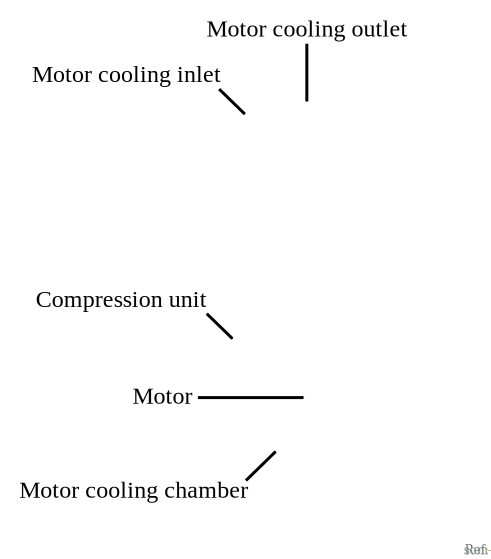
\includegraphics[width=6cm]{awp-motor-cooling-io}
  \caption{AWP motor cooling inlet/outlet (heating mode)}
  \label{fig:awp_motor_cooling_io}
\end{figure}

\section{Sensors}
\label[secinapp]{sec:awp-sensors}

The thermocouples are fastened on the pipes and fittings using Serto
male union parts\footnotep{Serto male metric union M5 SO-41124-2-M5,
  for the 2mm-diameter-thermocouples. For the
  0.5mm-diameter-thermocouples, an adaptation sleeve in Teflon, with
  conical shapes, was manufactured by the EPFL mechanical
  workshop. They were adapted, then, to the Serto fittings.}.

\Cref{fig:awp-electromagnetic-perturbation-P} illustrates what is
observed on \cref{fig:awp-sh-too-low-ev-sh-with-plate}.

\begin{figure}[htbp]
  \centering
  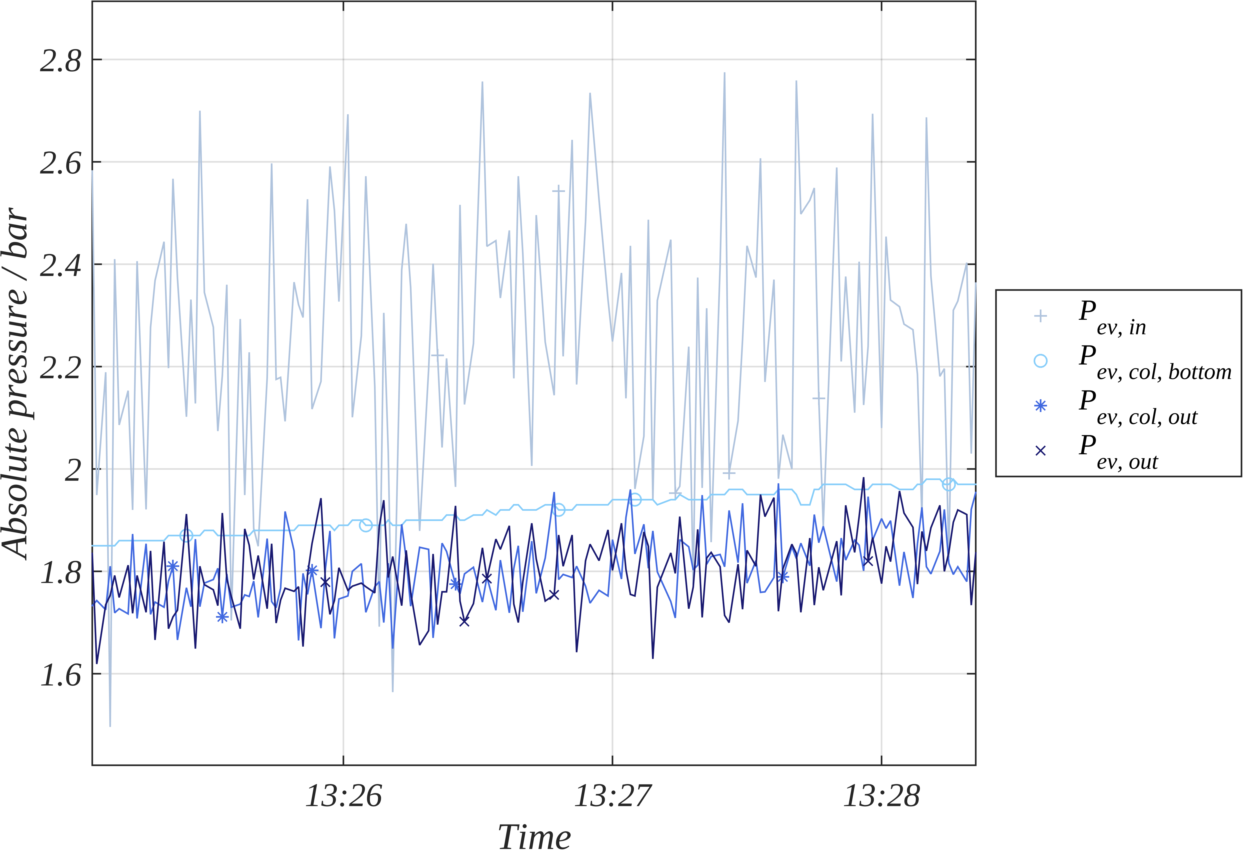
\includegraphics[width=10cm]{awp-magnetic-perturbation-02}
  \caption{Electro-magnetic perturbation of pressure sensors signals}
  \label{fig:awp-electromagnetic-perturbation-P}
\end{figure}

\begin{figure}
  \centering
  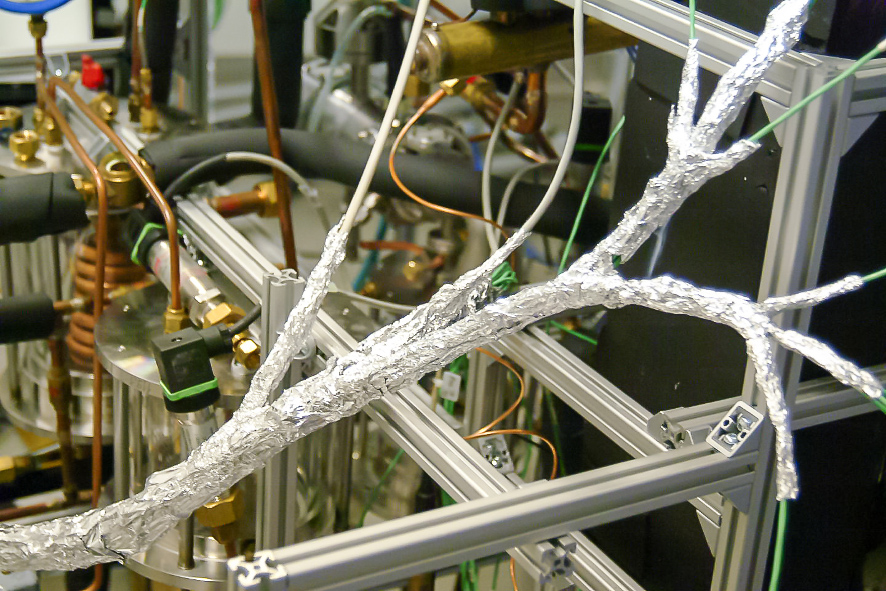
\includegraphics[width=10cm]{DSCF0219}
  \caption{Extra shielding of the AWP sensor cables}
  \label{fig:awp-alu-sheets-shield}
\end{figure}


\FloatBarrier

\bibliographystyle{plainnat}
\bibliography{main}
\label[secinapp]{sec:awp-components-refs}
